\section{Results and Discussion}
\label{sec:results}

\begin{figure*}[t]
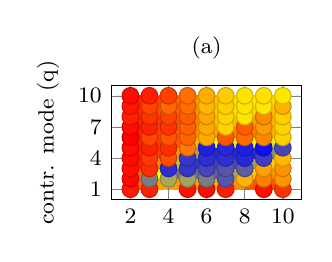
\begin{tikzpicture}
\begin{axis}
[
width=0.33\textwidth,
height=0.25\textwidth,
style={font=\footnotesize},
grid=major,
grid style={dotted},
align=center,
%xlabel={tensor order},
ylabel={contr. mode (q)},
title={{(a)}}, %  bgemm, asymmetric
scaled ticks=false,
zlabel={GFlops},
view={0}{90}, 
ytick={1,4,7,10},
xtick={2,4,6,8,10},
xmin=1, xmax=11,
ymin=0, ymax=11,
try min ticks=8,
zmin=300, zmax=2300,
point meta min=300, point meta max=2300,
colormap/hot, 
samples=50,
%colorbar sampled,
%colorbar/width=0.2cm,
%colorbar style={
%	point meta min=300, point meta max=2300,
%	samples=50,
%	font=\footnotesize,
%	ytick={300,1300,2300},
%	yticklabels={0.3,1.3,2.3},
%	%title={\scriptsize Gflops},
%	%ylabel={\scriptsize Gflops},
%}
]
%\addplot3[mesh, scatter,samples=50,shader=interp]
%\addplot3[only marks, mesh, scatter,scatter src=z,samples=50,] % z buffer=sort, scatter src=z,
\addplot3[contour filled={number=100},scatter,shader=flat,samples=50]
%\addplot3+[mesh,scatter,shader=flat corner,samples=50, only marks, mark size=2]
coordinates{
	
(2.000,1.000,2142.734) (2.000,2.000,2241.014) (2.000,3.000,2205.546) (2.000,4.000,2226.263) (2.000,5.000,2232.877) (2.000,6.000,2281.816) (2.000,7.000,2222.317) (2.000,8.000,2122.831) (2.000,9.000,2166.437) (2.000,10.000,2231.354) 

(3.000,1.000,2104.803) (3.000,2.000,620.292) (3.000,3.000,2053.810) (3.000,4.000,1989.460) (3.000,5.000,2100.108) (3.000,6.000,1923.866) (3.000,7.000,2109.798) (3.000,8.000,2032.918) (3.000,9.000,1931.835) (3.000,10.000,2137.550) 

(4.000,1.000,2303.560) (4.000,2.000,742.055) (4.000,3.000,436.752) (4.000,4.000,1889.266) (4.000,5.000,2050.848) (4.000,6.000,1845.429) (4.000,7.000,2029.757) (4.000,8.000,1947.246) (4.000,9.000,1753.968) (4.000,10.000,1945.836) 

(5.000,1.000,2197.949) (5.000,2.000,727.736) (5.000,3.000,441.734) (5.000,4.000,458.055) (5.000,5.000,1643.657) (5.000,6.000,1763.676) (5.000,7.000,1793.195) (5.000,8.000,1799.906) (5.000,9.000,1726.622) (5.000,10.000,1710.693) 

(6.000,1.000,2225.857) (6.000,2.000,621.489) (6.000,3.000,489.438) (6.000,4.000,435.500) (6.000,5.000,386.554) (6.000,6.000,1410.907) (6.000,7.000,1419.437) (6.000,8.000,1428.795) (6.000,9.000,1330.280) (6.000,10.000,1386.923) 

(7.000,1.000,2137.668) (7.000,2.000,530.662) (7.000,3.000,532.587) (7.000,4.000,439.307) (7.000,5.000,400.923) (7.000,6.000,1835.402) (7.000,7.000,1186.143) (7.000,8.000,1195.514) (7.000,9.000,1211.432) (7.000,10.000,1230.143) 

(8.000,1.000,2411.000) (8.000,2.000,1340.829) (8.000,3.000,546.729) (8.000,4.000,405.255) (8.000,5.000,381.061) (8.000,6.000,1724.053) (8.000,7.000,1816.684) (8.000,8.000,1103.276) (8.000,9.000,1109.365) (8.000,10.000,1119.582) 

(9.000,1.000,2215.896) (9.000,2.000,1637.409) (9.000,3.000,1448.314) (9.000,4.000,477.752) (9.000,5.000,353.959) (9.000,6.000,1596.361) (9.000,7.000,1496.308) (9.000,8.000,1566.431) (9.000,9.000,1085.107) (9.000,10.000,1135.908) 

(10.000,1.000,2011.147) (10.000,2.000,1504.412) (10.000,3.000,1538.421) (10.000,4.000,1335.732) (10.000,5.000,483.993) (10.000,6.000,1202.734) (10.000,7.000,1197.316) (10.000,8.000,1213.834) (10.000,9.000,1362.208) (10.000,10.000,1087.708)


};
\end{axis}
\end{tikzpicture}
\hfill
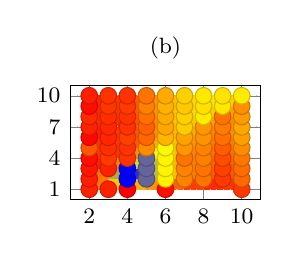
\begin{tikzpicture}
\begin{axis}
[
width=0.33\textwidth,
height=0.25\textwidth,
style={font=\footnotesize},
grid=major,
grid style={dotted},
align=center,
%xlabel={tensor order},
%ylabel={contr. mode (q)},
title={{(b)}}, %  ompfor<2d-slice> ttm<par-loops,seq-blas,$q$-slice>, asymmetric
scaled ticks=false,
zlabel={GFlops},
view={0}{90}, 
%view={-45}{45}, 
ytick={1,4,7,10},
xtick={2,4,6,8,10},
xmin=1, xmax=11,
ymin=0, ymax=11,
try min ticks=8,
zmin=300, zmax=2300,
point meta min=300, point meta max=2300,
colormap/hot, 
samples=50,
%colorbar sampled,
%colorbar/width=0.2cm,
%colorbar style={
%	point meta min=300, point meta max=2300,
%	samples=50,
%	font=\footnotesize,
%	ytick={300,1300,2300},
%	yticklabels={0.3,1.3,2.3},
%	%title={\scriptsize Gflops},
%	%ylabel={\scriptsize Gflops},
%}
]
%\addplot3[mesh, scatter,samples=50,shader=interp]
%\addplot3[only marks, mesh, scatter,scatter src=z,samples=50,] % z buffer=sort, scatter src=z,
\addplot3[contour filled={number=100},scatter,shader=flat,samples=50]
%\addplot3+[mesh,scatter,shader=flat corner,samples=50, only marks, mark size=2]
coordinates{

(2.000,1.000,2107.002) (2.000,2.000,2127.162) (2.000,3.000,2176.298) (2.000,4.000,2215.649) (2.000,5.000,1837.632) (2.000,6.000,2241.609) (2.000,7.000,2101.558) (2.000,8.000,2075.436) (2.000,9.000,2236.130) (2.000,10.000,2133.353) 

(3.000,1.000,2119.523) (3.000,2.000,167.437) (3.000,3.000,2112.420) (3.000,4.000,1989.285) (3.000,5.000,2041.921) (3.000,6.000,2084.201) (3.000,7.000,2080.454) (3.000,8.000,2046.614) (3.000,9.000,2013.009) (3.000,10.000,2024.421) 

(4.000,1.000,2285.299) (4.000,2.000,314.287) (4.000,3.000,311.849) (4.000,4.000,2011.869) (4.000,5.000,2039.029) (4.000,6.000,1944.642) (4.000,7.000,2023.178) (4.000,8.000,2033.385) (4.000,9.000,1992.379) (4.000,10.000,2039.303) 

(5.000,1.000,2475.804) (5.000,2.000,568.291) (5.000,3.000,562.230) (5.000,4.000,562.587) (5.000,5.000,1564.667) (5.000,6.000,1756.890) (5.000,7.000,1791.524) (5.000,8.000,1712.024) (5.000,9.000,1626.887) (5.000,10.000,1695.764) 

(6.000,1.000,2218.038) (6.000,2.000,1025.980) (6.000,3.000,1034.039) (6.000,4.000,1026.350) (6.000,5.000,945.367) (6.000,6.000,1340.191) (6.000,7.000,1422.937) (6.000,8.000,1402.244) (6.000,9.000,1375.707) (6.000,10.000,1411.432) 

(7.000,1.000,2307.246) (7.000,2.000,1602.074) (7.000,3.000,1617.348) (7.000,4.000,1682.539) (7.000,5.000,1516.443) (7.000,6.000,1446.511) (7.000,7.000,1229.353) (7.000,8.000,1202.606) (7.000,9.000,1245.855) (7.000,10.000,1211.880) 

(8.000,1.000,2441.539) (8.000,2.000,1699.771) (8.000,3.000,1686.405) (8.000,4.000,1622.372) (8.000,5.000,1600.438) (8.000,6.000,1530.707) (8.000,7.000,1508.466) (8.000,8.000,1073.808) (8.000,9.000,1123.363) (8.000,10.000,1096.486) 

(9.000,1.000,2330.060) (9.000,2.000,1985.056) (9.000,3.000,1941.312) (9.000,4.000,1892.533) (9.000,5.000,1805.699) (9.000,6.000,1706.515) (9.000,7.000,1658.818) (9.000,8.000,1693.350) (9.000,9.000,1093.684) (9.000,10.000,1112.530) 

(10.000,1.000,1988.818) (10.000,2.000,1750.516) (10.000,3.000,1728.226) (10.000,4.000,1678.568) (10.000,5.000,1576.395) (10.000,6.000,1476.492) (10.000,7.000,1429.733) (10.000,8.000,1496.574) (10.000,9.000,1557.162) (10.000,10.000,1068.719) 


};
\end{axis}
\end{tikzpicture}
\hfill
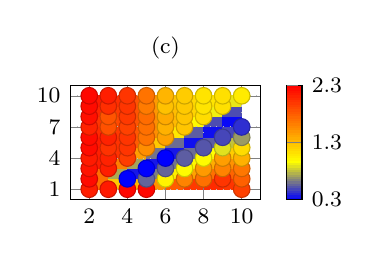
\begin{tikzpicture}
\begin{axis}
[
width=0.33\textwidth,
height=0.25\textwidth,
style={font=\footnotesize},
grid=major,
grid style={dotted},
align=center,
%xlabel={tensor order},
%ylabel={contr. mode (q)},
title={{(c)}}, %  ompfor<qd-slice> ttm<par-loops,seq-blas,$q$-slice>, asymmetric
scaled ticks=false,
zlabel={GFlops},
view={0}{90}, 
%view={-45}{45}, 
ytick={1,4,7,10},
xtick={2,4,6,8,10},
%xmin=2, xmax=10,
%ymin=1, ymax=10,
xmin=1, xmax=11,
ymin=0, ymax=11,
try min ticks=8,
zmin=300, zmax=2300,
point meta min=300, point meta max=2300,
%colormap/jet, 
colormap/hot, 
%colormap/blackwhite,
%colormap={whiteblack}{indices of colormap={\pgfplotscolormaplastindexof{blackwhite},...,0 of blackwhite}},
samples=50,
%colormap access=piecewise const,
colorbar sampled,
colorbar/width=0.2cm,
colorbar style={
	point meta min=300, point meta max=2300,
	samples=50,
	font=\footnotesize,
	ytick={300,1300,2300},
	yticklabels={0.3,1.3,2.3},
	%title={\scriptsize Gflops},
	%ylabel={\scriptsize Gflops},
}
]
%\addplot3[mesh, scatter,samples=50,shader=interp]
%\addplot3[only marks, mesh, scatter,scatter src=z,samples=50,] % z buffer=sort, scatter src=z,
\addplot3[contour filled={number=100},scatter,shader=flat,samples=50]
%\addplot3+[mesh,scatter,shader=flat corner,samples=50, only marks, mark size=2]
coordinates{

(2.000,1.000,2134.021) (2.000,2.000,2224.864) (2.000,3.000,2184.477) (2.000,4.000,2142.541) (2.000,5.000,2229.439) (2.000,6.000,2238.772) (2.000,7.000,2105.091) (2.000,8.000,2201.214) (2.000,9.000,2232.448) (2.000,10.000,2240.926) 

(3.000,1.000,2146.896) (3.000,2.000,167.544) (3.000,3.000,2121.476) (3.000,4.000,2105.304) (3.000,5.000,2027.717) (3.000,6.000,2104.722) (3.000,7.000,1866.561) (3.000,8.000,1855.180) (3.000,9.000,2041.894) (3.000,10.000,2122.692) 

(4.000,1.000,2244.985) (4.000,2.000,313.766) (4.000,3.000,167.879) (4.000,4.000,1973.457) (4.000,5.000,2013.391) (4.000,6.000,2010.678) (4.000,7.000,1949.136) (4.000,8.000,1989.844) (4.000,9.000,2017.192) (4.000,10.000,2015.899) 

(5.000,1.000,2250.694) (5.000,2.000,574.277) (5.000,3.000,315.908) (5.000,4.000,166.343) (5.000,5.000,1559.782) (5.000,6.000,1688.138) (5.000,7.000,1711.412) (5.000,8.000,1721.389) (5.000,9.000,1653.587) (5.000,10.000,1691.902) 

(6.000,1.000,2403.465) (6.000,2.000,1026.371) (6.000,3.000,576.699) (6.000,4.000,312.020) (6.000,5.000,160.917) (6.000,6.000,1443.174) (6.000,7.000,1370.699) (6.000,8.000,1414.204) (6.000,9.000,1283.900) (6.000,10.000,1351.446) 

(7.000,1.000,2305.894) (7.000,2.000,1613.830) (7.000,3.000,988.435) (7.000,4.000,554.792) (7.000,5.000,290.305) (7.000,6.000,157.356) (7.000,7.000,1270.432) (7.000,8.000,1266.914) (7.000,9.000,1255.620) (7.000,10.000,1224.914) 

(8.000,1.000,2437.239) (8.000,2.000,1706.219) (8.000,3.000,1489.110) (8.000,4.000,999.755) (8.000,5.000,531.137) (8.000,6.000,280.182) (8.000,7.000,148.892) (8.000,8.000,1156.621) (8.000,9.000,1110.478) (8.000,10.000,1116.944) 

(9.000,1.000,2355.395) (9.000,2.000,2003.839) (9.000,3.000,1603.752) (9.000,4.000,1477.309) (9.000,5.000,887.839) (9.000,6.000,492.554) (9.000,7.000,262.294) (9.000,8.000,150.408) (9.000,9.000,1129.997) (9.000,10.000,1121.143) 

(10.000,1.000,1944.959) (10.000,2.000,1789.054) (10.000,3.000,1665.441) (10.000,4.000,1375.291) (10.000,5.000,1147.731) (10.000,6.000,715.205) (10.000,7.000,422.658) (10.000,8.000,236.076) (10.000,9.000,136.520) (10.000,10.000,1078.495) 


};
\end{axis}
\end{tikzpicture}


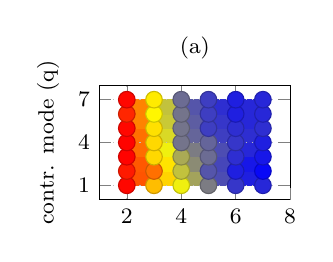
\begin{tikzpicture}
\begin{axis}
[
width=0.33\textwidth,
height=0.25\textwidth,
style={font=\footnotesize},
grid=major,
grid style={dotted},
align=center,
%xlabel={tensor order},
ylabel={contr. mode (q)},
title={{(a)}}, %  bgemm, asymmetric
scaled ticks=false,
zlabel={GFlops},
view={0}{90}, 
ytick={1,4,7,10},
xtick={2,4,6,8},
xmin=1, xmax=8,
ymin=0, ymax=8,
try min ticks=8,
zmin=0, zmax=2600,
point meta min=0, point meta max=2600,
colormap/hot, 
samples=50,
%colorbar sampled,
%colorbar/width=0.2cm,
%colorbar style={
%	point meta min=300, point meta max=2300,
%	samples=50,
%	font=\footnotesize,
%	ytick={300,1300,2300},
%	yticklabels={0.3,1.3,2.3},
%	%title={\scriptsize Gflops},
%	%ylabel={\scriptsize Gflops},
%}
]
%\addplot3[mesh, scatter,samples=50,shader=interp]
%\addplot3[only marks, mesh, scatter,scatter src=z,samples=50,] % z buffer=sort, scatter src=z,
\addplot3[contour filled={number=100},scatter,shader=flat,samples=50]
%\addplot3+[mesh,scatter,shader=flat corner,samples=50, only marks, mark size=2]
coordinates{

(2.000,1.000,2527.923) (2.000,2.000,2398.051) (2.000,3.000,2573.521) (2.000,4.000,2570.296) (2.000,5.000,2540.651) (2.000,6.000,2326.903) (2.000,7.000,2545.629) 

(3.000,1.000,1312.517) (3.000,2.000,1835.211) (3.000,3.000,1133.124) (3.000,4.000,1120.384) (3.000,5.000,1066.704) (3.000,6.000,915.932) (3.000,7.000,997.168) 

(4.000,1.000,825.045) (4.000,2.000,655.270) (4.000,3.000,579.750) (4.000,4.000,390.794) (4.000,5.000,411.134) (4.000,6.000,409.619) (4.000,7.000,375.457) 

(5.000,1.000,420.343) (5.000,2.000,308.678) (5.000,3.000,377.118) (5.000,4.000,348.232) (5.000,5.000,216.877) (5.000,6.000,232.073) (5.000,7.000,218.457) 

(6.000,1.000,206.774) (6.000,2.000,119.299) (6.000,3.000,167.691) (6.000,4.000,183.571) (6.000,5.000,179.989) (6.000,6.000,126.876) (6.000,7.000,128.135) 

(7.000,1.000,150.823) (7.000,2.000,33.170) (7.000,3.000,83.979) (7.000,4.000,128.221) (7.000,5.000,157.368) (7.000,6.000,143.557) (7.000,7.000,133.647) 


};
\end{axis}
\end{tikzpicture}
\hfill
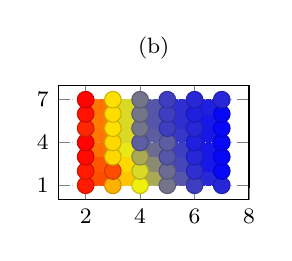
\begin{tikzpicture}
\begin{axis}
[
width=0.33\textwidth,
height=0.25\textwidth,
style={font=\footnotesize},
grid=major,
grid style={dotted},
align=center,
%xlabel={tensor order},
%ylabel={contr. mode (q)},
title={{(b)}}, %  ompfor<2d-slice> ttm<par-loops,seq-blas,$q$-slice>, asymmetric
scaled ticks=false,
zlabel={GFlops},
view={0}{90}, 
%view={-45}{45}, 
ytick={1,4,7,10},
xtick={2,4,6,8},
xmin=1, xmax=8,
ymin=0, ymax=8,
try min ticks=8,
zmin=0, zmax=2600,
point meta min=0, point meta max=2600,
colormap/hot, 
samples=50,
%colorbar sampled,
%colorbar/width=0.2cm,
%colorbar style={
%	point meta min=300, point meta max=2300,
%	samples=50,
%	font=\footnotesize,
%	ytick={300,1300,2300},
%	yticklabels={0.3,1.3,2.3},
%	%title={\scriptsize Gflops},
%	%ylabel={\scriptsize Gflops},
%}
]
%\addplot3[mesh, scatter,samples=50,shader=interp]
%\addplot3[only marks, mesh, scatter,scatter src=z,samples=50,] % z buffer=sort, scatter src=z,
\addplot3[contour filled={number=100},scatter,shader=flat,samples=50]
%\addplot3+[mesh,scatter,shader=flat corner,samples=50, only marks, mark size=2]
coordinates{

(2.000,1.000,2394.429) (2.000,2.000,2411.386) (2.000,3.000,2508.441) (2.000,4.000,2549.390) (2.000,5.000,2334.831) (2.000,6.000,2454.725) (2.000,7.000,2556.685) 

(3.000,1.000,1395.054) (3.000,2.000,2055.946) (3.000,3.000,1121.102) (3.000,4.000,1120.659) (3.000,5.000,1089.377) (3.000,6.000,1102.959) (3.000,7.000,1078.957) 

(4.000,1.000,819.991) (4.000,2.000,729.342) (4.000,3.000,579.869) (4.000,4.000,334.133) (4.000,5.000,390.153) (4.000,6.000,407.045) (4.000,7.000,394.057) 

(5.000,1.000,414.803) (5.000,2.000,369.532) (5.000,3.000,295.077) (5.000,4.000,318.473) (5.000,5.000,209.139) (5.000,6.000,214.825) (5.000,7.000,223.888) 

(6.000,1.000,208.097) (6.000,2.000,156.950) (6.000,3.000,141.868) (6.000,4.000,119.992) (6.000,5.000,134.757) (6.000,6.000,126.271) (6.000,7.000,133.034) 

(7.000,1.000,151.228) (7.000,2.000,27.225) (7.000,3.000,30.634) (7.000,4.000,31.221) (7.000,5.000,30.322) (7.000,6.000,31.152) (7.000,7.000,133.496) 


};
\end{axis}
\end{tikzpicture}
\hfill
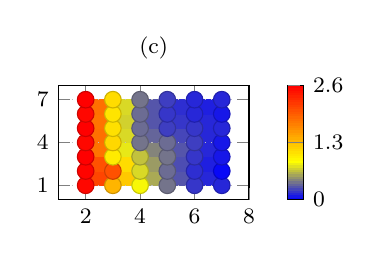
\begin{tikzpicture}
\begin{axis}
[
width=0.33\textwidth,
height=0.25\textwidth,
style={font=\footnotesize},
grid=major,
grid style={dotted},
align=center,
%xlabel={tensor order},
%ylabel={contr. mode (q)},
title={{(c)}}, %  ompfor<qd-slice> ttm<par-loops,seq-blas,$q$-slice>, asymmetric
scaled ticks=false,
zlabel={GFlops},
view={0}{90}, 
ytick={1,4,7,10},
xtick={2,4,6,8},
xmin=1, xmax=8,
ymin=0, ymax=8,
try min ticks=8,
zmin=0, zmax=2600,
point meta min=0, point meta max=2600,
%colormap/jet, 
colormap/hot, 
%colormap/blackwhite,
%colormap={whiteblack}{indices of colormap={\pgfplotscolormaplastindexof{blackwhite},...,0 of blackwhite}},
samples=50,
%colormap access=piecewise const,
colorbar sampled,
colorbar/width=0.2cm,
colorbar style={
point meta min=0, point meta max=2600,
samples=50,
font=\footnotesize,
ytick={0,1300,2600},
yticklabels={0,1.3,2.6},
%title={\scriptsize Gflops},
%ylabel={\scriptsize Gflops},
}
]
%\addplot3[mesh, scatter,samples=50,shader=interp]
%\addplot3[only marks, mesh, scatter,scatter src=z,samples=50,] % z buffer=sort, scatter src=z,
\addplot3[contour filled={number=100},scatter,shader=flat,samples=50]
%\addplot3+[mesh,scatter,shader=flat corner,samples=50, only marks, mark size=2]
coordinates{

(2.000,1.000,2536.639) (2.000,2.000,2549.050) (2.000,3.000,2598.729) (2.000,4.000,2525.744) (2.000,5.000,2590.830) (2.000,6.000,2544.134) (2.000,7.000,2589.762) 

(3.000,1.000,1375.656) (3.000,2.000,2048.636) (3.000,3.000,1013.687) (3.000,4.000,1124.134) (3.000,5.000,1075.977) (3.000,6.000,1052.382) (3.000,7.000,1098.544) 

(4.000,1.000,833.978) (4.000,2.000,732.322) (4.000,3.000,660.833) (4.000,4.000,413.827) (4.000,5.000,368.029) (4.000,6.000,382.244) (4.000,7.000,404.286) 

(5.000,1.000,415.086) (5.000,2.000,368.007) (5.000,3.000,411.465) (5.000,4.000,371.633) (5.000,5.000,212.971) (5.000,6.000,198.100) (5.000,7.000,222.798) 

(6.000,1.000,206.159) (6.000,2.000,156.941) (6.000,3.000,192.783) (6.000,4.000,217.075) (6.000,5.000,186.601) (6.000,6.000,132.454) (6.000,7.000,130.229) 

(7.000,1.000,150.869) (7.000,2.000,27.399) (7.000,3.000,91.695) (7.000,4.000,85.698) (7.000,5.000,132.060) (7.000,6.000,86.740) (7.000,7.000,146.783) 


};
\end{axis}
\end{tikzpicture}

\caption{%
\footnotesize %
Performance maps in double-precision Tflops/s of the proposed tensor-times-matrix algorithms with varying tensor orders $p$  and contraction modes $q$. 
Tensors are asymmetrically-shaped on the upper plots and symmetrically-shaped on the lower plots.
The algorithm of 
(a) and (e) executes \tf{gemm\_batch} with subtensors, %
(b) and (e) parallel loops over single-threaded \tf{gemm} with tensor slices, %
(c) and (f) parallel loop over single-threaded \tf{gemm} with subtensors.
\label{performance.tlib.contour}
}
\end{figure*}


\begin{figure*}[t]
\input{figures/performance.tlib.case8}
\caption{ %
\footnotesize%
Box plots visualizing performance statics in double-precision Tflops/s of the proposed tensor-times-matrix algorithms for the 8-th case.
Tensors are asymmetrically-shaped on the left plot and symmetrically-shaped on the right plot.
The Algorithm of
(a) executes \tf{gemm\_batch} with subtensors,
(b) and (e) sequential loops over multi-threaded \tf{gemm}, %
(c) and (f) parallel loops over single-threaded \tf{gemm}, %
(d) and (g) parallel loops over multi-threaded \tf{gemm}.
The algorithms (b,c,d) and (e,f,g) are executed with tensor slices or subtensors, respectively.
%(a) \texttt{tlib<bgemm,subtensor,all>}, (b) \texttt{tlib<tgemm,slice>}, (c) \texttt{tlib<ompfor,slice,all>}, (d) \texttt{tlib<ompfor,tgemm,slice,all>}, (e) \texttt{tlib<tgemm,subtensor>}, (f) \texttt{tlib<ompfor,subtensor,all>}, (g) \texttt{tlib<ompfor,tgemm,subtensor,outer>}, Tensor elements are \textbf{64-Bit floating point} numbers.\\
%The dashed horizontal line denotes the measured upper bound of the available throughput.
%The horizontal lines with a dot are the median throughput of the \tf{libstdc++}.
%Numbers below the lower whisker are the median values of the corresponding boxes.
}
\label{fig:performance.tlib.case8}
\end{figure*}


\begin{figure*}[t]
\begin{tikzpicture}
\begin{axis}[
boxplot/draw direction=y,
width=0.37\textwidth,
height=0.3\textheight,
style={font=\footnotesize},
grid=major,
grid style={dotted},
align=center,
xlabel={$k$-order layout},
ylabel={TFlops},
ylabel near ticks,
%title={Performance (Tflops/s)},
xtick={1,2,3,4,5,6,7},
xticklabels={1,2,3,4,5,6,7},
ymin=0,
ymax=200,
ytick={0,100,200},
yticklabels={0,0.1,0.2},
cycle list={{black}},
boxplot/variable width,
boxplot/box extend=0.5,
boxplot/every box/.style={fill=black,thick},
boxplot/every median/.style={draw=white,thin},
]
\addplot+[boxplot prepared={lower whisker = 12.953287, lower quartile = 60.316441, median = 75.006325, upper quartile = 89.433827, upper whisker = 117.121454} ] coordinates{};
\addplot+[boxplot prepared={lower whisker = 12.640045, lower quartile = 48.857803, median = 71.928801, upper quartile = 83.642690, upper whisker = 129.266128} ] coordinates{};
\addplot+[boxplot prepared={lower whisker = 11.285366, lower quartile = 38.052710, median = 47.911392, upper quartile = 58.133262, upper whisker = 82.945640} ] coordinates{};
\addplot+[boxplot prepared={lower whisker = 15.226172, lower quartile = 57.231846, median = 80.633181, upper quartile = 93.816564, upper whisker = 183.850079} ] coordinates{};
\addplot+[boxplot prepared={lower whisker = 14.986315, lower quartile = 49.549662, median = 65.947492, upper quartile = 82.637276, upper whisker = 134.213232} ] coordinates{};
\addplot+[boxplot prepared={lower whisker = 10.126218, lower quartile = 48.886168, median = 65.468008, upper quartile = 78.704242, upper whisker = 142.986427} ] coordinates{};
\addplot+[boxplot prepared={lower whisker = 9.920391, lower quartile = 46.556304, median = 53.812431, upper quartile = 67.449759, upper whisker = 97.531103} ] coordinates{};
\end{axis}
\end{tikzpicture}
\begin{tikzpicture}
\begin{axis}[
boxplot/draw direction=y,
width=0.37\textwidth,
height=0.3\textheight,
style={font=\footnotesize},
grid=major,
grid style={dotted},
align=center,
xlabel={$k$-order layout},
%xlabel={Function},
%ylabel={GFlops},
%ylabel near ticks,
%title={Performance (Tflops/s)},
xtick={1,2,3,4,5,6,7},
xticklabels={1,2,3,4,5,6,7},
ymin=0,
ymax=200,
ytick={0,100,200},
yticklabels={0,0.1,0.2},
cycle list={{black}},
boxplot/variable width,
boxplot/box extend=0.5,
boxplot/every box/.style={fill=black,thick},
boxplot/every median/.style={draw=white,thin},
]
\addplot+[boxplot prepared={lower whisker = 9.972735, lower quartile = 50.927006, median = 64.426586, upper quartile = 79.210059, upper whisker = 102.890428} ] coordinates{};
\addplot+[boxplot prepared={lower whisker = 9.924992, lower quartile = 53.823097, median = 66.585367, upper quartile = 76.424392, upper whisker = 126.976560} ] coordinates{};
\addplot+[boxplot prepared={lower whisker = 9.870402, lower quartile = 40.752707, median = 53.587394, upper quartile = 66.305725, upper whisker = 101.453234} ] coordinates{};
\addplot+[boxplot prepared={lower whisker = 14.708473, lower quartile = 68.924818, median = 80.163598, upper quartile = 97.636473, upper whisker = 172.275314} ] coordinates{};
\addplot+[boxplot prepared={lower whisker = 13.901132, lower quartile = 56.095772, median = 71.850410, upper quartile = 87.921333, upper whisker = 133.760673} ] coordinates{};
\addplot+[boxplot prepared={lower whisker = 9.637782, lower quartile = 64.849736, median = 77.669292, upper quartile = 95.936764, upper whisker = 142.318829} ] coordinates{};
\addplot+[boxplot prepared={lower whisker = 8.748652, lower quartile = 51.209701, median = 67.054182, upper quartile = 87.504879, upper whisker = 115.340741} ] coordinates{};
\end{axis}
\end{tikzpicture}
\begin{tikzpicture}
\begin{axis}[
boxplot/draw direction=y,
width=0.37\textwidth,
height=0.3\textheight,
style={font=\footnotesize},
grid=major,
grid style={dotted},
align=center,
xlabel={$k$-order layout},
%xlabel={Function},
%ylabel={Gflops},
%ylabel near ticks,
%title={},
xtick={1,2,3,4,5,6,7},
xticklabels={1,2,3,4,5,6,7},
ymin=0,
ymax=200,
ytick={0,100,200},
yticklabels={0,0.1,0.2},
cycle list={{black}},
boxplot/variable width,
boxplot/box extend=0.5,
boxplot/every box/.style={fill=black,thick},
boxplot/every median/.style={draw=white,thin},
]
\addplot+[boxplot prepared={lower whisker = 7.132722, lower quartile = 11.482166, median = 22.426546, upper quartile = 34.658759, upper whisker = 102.949746} ] coordinates{};
\addplot+[boxplot prepared={lower whisker = 6.479361, lower quartile = 14.151379, median = 27.103188, upper quartile = 40.479719, upper whisker = 97.896991} ] coordinates{};
\addplot+[boxplot prepared={lower whisker = 6.588109, lower quartile = 14.269192, median = 27.672456, upper quartile = 47.110864, upper whisker = 76.267702} ] coordinates{};
\addplot+[boxplot prepared={lower whisker = 10.384620, lower quartile = 19.559000, median = 36.409643, upper quartile = 56.801437, upper whisker = 115.192574} ] coordinates{};
\addplot+[boxplot prepared={lower whisker = 9.428007, lower quartile = 18.814353, median = 35.234564, upper quartile = 50.282299, upper whisker = 93.764754} ] coordinates{};
\addplot+[boxplot prepared={lower whisker = 8.495888, lower quartile = 18.190874, median = 34.228483, upper quartile = 68.448730, upper whisker = 110.241613} ] coordinates{};
\addplot+[boxplot prepared={lower whisker = 7.307545, lower quartile = 16.797509, median = 31.145092, upper quartile = 47.293157, upper whisker = 95.475018} ] coordinates{};
\end{axis}
\end{tikzpicture}
\caption{ %
\footnotesize%
Box plots visualizing performance statics in double-precision Tflops/s of a tensor-times-matrix algorithm for linear $k$-order tensor formats.
The algorithm loops over single-threaded \tf{gemm} with tensor slices with asymmetrically-shaped tensors on the left plot and with subtensors with symmetrically-shaped tensors on the right plot.
Box plot number $k$ denotes the utilized $k$-order storage.
}
\label{fig:performance.tlib.format}
\end{figure*}

\begin{figure*}[t]
\centering
\tikzset{every mark/.append style={scale=1.5}}
\begin{tikzpicture}
\begin{axis}[
height=0.3\textheight,
width=0.5\textwidth,
style={font=\footnotesize},
grid=major,
grid style={dotted},
align=center,
xlabel={Tflops/s},
ylabel={Cumulative Probability},
ylabel near ticks,
%title={Empirical CDF},
xtick={0,200,400,600,800,1000,1200},
xticklabels={0,0.2,0.4,0.6,0.8,1.0,1.2},
ytick={0,0.25,0.5,0.75,1},
yticklabels={0,0.25,0.5,0.75,1},
mark repeat={16},
cycle list name=my exotic compare 1,
]
\addplot%%+[const plo, line width=1,mark options={scale=2}]
coordinates{(126.866,0.000) (127.677,0.006) (128.446,0.012) (247.352,0.019) (250.808,0.025) (252.096,0.031) (254.061,0.037) (321.953,0.043) (337.772,0.049) (357.481,0.056) (412.844,0.062) (450.627,0.068) (455.588,0.074) (464.506,0.080) (468.515,0.086) (474.322,0.093) (477.948,0.099) (480.605,0.105) (482.078,0.111) (483.738,0.117) (487.720,0.123) (489.836,0.130) (492.948,0.136) (494.196,0.142) (499.662,0.148) (506.376,0.154) (510.779,0.160) (515.783,0.167) (520.894,0.173) (525.108,0.179) (527.089,0.185) (532.859,0.191) (538.446,0.198) (544.298,0.204) (551.766,0.210) (557.982,0.216) (563.185,0.222) (566.275,0.228) (570.012,0.235) (571.158,0.241) (576.303,0.247) (578.059,0.253) (579.951,0.259) (585.897,0.265) (590.075,0.272) (599.910,0.278) (626.566,0.284) (634.520,0.290) (646.815,0.296) (656.521,0.302) (661.127,0.309) (676.246,0.315) (688.133,0.321) (694.718,0.327) (699.650,0.333) (701.233,0.340) (712.888,0.346) (720.135,0.352) (725.611,0.358) (730.510,0.364) (733.161,0.370) (742.291,0.377) (745.256,0.383) (749.667,0.389) (752.126,0.395) (755.487,0.401) (758.905,0.407) (764.158,0.414) (765.321,0.420) (767.475,0.426) (768.327,0.432) (768.950,0.438) (772.050,0.444) (774.813,0.451) (776.982,0.457) (780.481,0.463) (782.098,0.469) (785.876,0.475) (792.372,0.481) (795.377,0.488) (796.955,0.494) (800.447,0.500) (803.250,0.506) (803.664,0.512) (806.341,0.519) (811.503,0.525) (816.284,0.531) (819.680,0.537) (824.874,0.543) (827.025,0.549) (829.100,0.556) (832.980,0.562) (836.813,0.568) (842.330,0.574) (843.940,0.580) (846.414,0.586) (848.632,0.593) (852.849,0.599) (854.707,0.605) (856.039,0.611) (859.563,0.617) (861.226,0.623) (866.165,0.630) (870.346,0.636) (870.870,0.642) (872.054,0.648) (873.365,0.654) (874.751,0.660) (876.361,0.667) (876.810,0.673) (877.733,0.679) (879.397,0.685) (880.678,0.691) (887.431,0.698) (889.518,0.704) (891.440,0.710) (893.903,0.716) (897.176,0.722) (904.337,0.728) (909.843,0.735) (914.883,0.741) (920.173,0.747) (923.853,0.753) (928.112,0.759) (931.755,0.765) (935.248,0.772) (936.845,0.778) (940.755,0.784) (941.951,0.790) (943.555,0.796) (946.601,0.802) (949.882,0.809) (957.884,0.815) (962.085,0.821) (965.307,0.827) (967.837,0.833) (974.058,0.840) (978.633,0.846) (983.465,0.852) (987.243,0.858) (993.242,0.864) (996.226,0.870) (1003.142,0.877) (1004.974,0.883) (1007.971,0.889) (1012.517,0.895) (1017.101,0.901) (1021.387,0.907) (1021.985,0.914) (1024.096,0.920) (1027.183,0.926) (1031.292,0.932) (1033.829,0.938) (1037.798,0.944) (1043.124,0.951) (1052.842,0.957) (1054.946,0.963) (1061.595,0.969) (1067.855,0.975) (1083.141,0.981) (1084.562,0.988) (1101.861,0.994) (1196.246,1.000) };
\label{coord:nonsymmetric.tlib.slice}
\addplot%%+[const plo %] %, line width=1,mark options={scale=2}]
coordinates{(39.550,0.000) (43.114,0.006) (70.346,0.012) (77.245,0.019) (79.570,0.025) (82.998,0.031) (114.998,0.037) (124.203,0.043) (139.879,0.049) (141.161,0.056) (141.686,0.062) (142.219,0.068) (161.072,0.074) (163.577,0.080) (174.279,0.086) (177.320,0.093) (178.717,0.099) (189.501,0.105) (193.508,0.111) (200.786,0.117) (204.520,0.123) (206.140,0.130) (207.206,0.136) (207.992,0.142) (214.557,0.148) (230.989,0.154) (235.636,0.160) (241.057,0.167) (244.729,0.173) (252.024,0.179) (255.686,0.185) (262.891,0.191) (266.307,0.198) (269.518,0.204) (271.184,0.210) (275.542,0.216) (280.687,0.222) (282.972,0.228) (286.782,0.235) (289.704,0.241) (291.724,0.247) (293.848,0.253) (295.234,0.259) (296.332,0.265) (297.270,0.272) (299.897,0.278) (302.580,0.284) (304.920,0.290) (306.456,0.296) (309.228,0.302) (312.951,0.309) (316.467,0.315) (318.262,0.321) (320.325,0.327) (323.732,0.333) (325.847,0.340) (327.659,0.346) (328.894,0.352) (331.488,0.358) (335.512,0.364) (338.491,0.370) (340.020,0.377) (346.111,0.383) (426.043,0.389) (432.175,0.395) (432.964,0.401) (433.759,0.407) (435.457,0.414) (436.158,0.420) (437.890,0.426) (444.750,0.432) (447.338,0.438) (455.131,0.444) (459.660,0.451) (464.654,0.457) (467.057,0.463) (474.215,0.469) (479.418,0.475) (481.156,0.481) (498.735,0.488) (501.447,0.494) (503.446,0.500) (504.986,0.506) (506.476,0.512) (507.895,0.519) (508.999,0.525) (510.054,0.531) (510.692,0.537) (512.411,0.543) (517.055,0.549) (518.668,0.556) (519.877,0.562) (520.706,0.568) (521.724,0.574) (523.148,0.580) (525.072,0.586) (527.088,0.593) (528.029,0.599) (528.514,0.605) (528.759,0.611) (529.588,0.617) (530.077,0.623) (530.762,0.630) (531.997,0.636) (532.778,0.642) (533.508,0.648) (533.947,0.654) (535.946,0.660) (536.735,0.667) (537.364,0.673) (538.118,0.679) (538.761,0.685) (539.418,0.691) (539.621,0.698) (540.086,0.704) (540.920,0.710) (541.705,0.716) (543.270,0.722) (544.178,0.728) (545.083,0.735) (545.682,0.741) (546.180,0.747) (546.887,0.753) (547.892,0.759) (549.700,0.765) (550.753,0.772) (551.629,0.778) (552.877,0.784) (554.315,0.790) (556.279,0.796) (557.919,0.802) (558.861,0.809) (560.317,0.815) (561.354,0.821) (564.021,0.827) (581.844,0.833) (588.241,0.840) (599.169,0.846) (604.501,0.852) (605.837,0.858) (611.346,0.864) (614.485,0.870) (618.627,0.877) (621.710,0.883) (624.989,0.889) (629.365,0.895) (635.038,0.901) (647.006,0.907) (657.583,0.914) (659.633,0.920) (661.884,0.926) (665.294,0.932) (668.252,0.938) (676.451,0.944) (679.661,0.951) (682.525,0.957) (693.310,0.963) (762.747,0.969) (772.635,0.975) (778.889,0.981) (798.965,0.988) (801.849,0.994) (812.196,1.000) };
\label{coord:nonsymmetric.tcl}
\addplot%%+[const plo %, line width=1,mark options={scale=2}]
coordinates{(225.666,0.000) (245.546,0.006) (251.857,0.012) (308.017,0.019) (320.236,0.025) (328.040,0.031) (330.465,0.037) (335.565,0.043) (340.689,0.049) (341.663,0.056) (346.282,0.062) (348.621,0.068) (350.505,0.074) (352.451,0.080) (353.014,0.086) (354.747,0.093) (356.749,0.099) (357.662,0.105) (358.948,0.111) (359.398,0.117) (360.653,0.123) (362.134,0.130) (362.583,0.136) (364.466,0.142) (365.263,0.148) (366.394,0.154) (367.236,0.160) (369.095,0.167) (370.649,0.173) (373.207,0.179) (373.564,0.185) (375.244,0.191) (376.006,0.198) (376.672,0.204) (378.452,0.210) (379.569,0.216) (380.310,0.222) (382.547,0.228) (384.196,0.235) (384.723,0.241) (386.180,0.247) (387.023,0.253) (387.320,0.259) (387.707,0.265) (388.128,0.272) (388.683,0.278) (389.504,0.284) (390.120,0.290) (391.187,0.296) (392.488,0.302) (393.816,0.309) (395.046,0.315) (397.090,0.321) (398.233,0.327) (399.301,0.333) (400.195,0.340) (400.850,0.346) (401.912,0.352) (402.635,0.358) (404.107,0.364) (404.997,0.370) (406.677,0.377) (406.980,0.383) (407.795,0.389) (407.831,0.395) (408.133,0.401) (409.897,0.407) (410.349,0.414) (410.648,0.420) (411.018,0.426) (411.560,0.432) (411.869,0.438) (412.260,0.444) (412.568,0.451) (413.224,0.457) (413.770,0.463) (413.909,0.469) (414.189,0.475) (414.335,0.481) (414.799,0.488) (415.123,0.494) (415.270,0.500) (415.644,0.506) (415.935,0.512) (416.203,0.519) (416.402,0.525) (416.736,0.531) (416.894,0.537) (417.341,0.543) (417.526,0.549) (417.984,0.556) (418.345,0.562) (418.756,0.568) (419.021,0.574) (419.900,0.580) (420.599,0.586) (421.253,0.593) (421.551,0.599) (422.684,0.605) (423.514,0.611) (423.835,0.617) (424.336,0.623) (424.463,0.630) (424.623,0.636) (425.859,0.642) (426.324,0.648) (427.562,0.654) (428.208,0.660) (429.116,0.667) (429.428,0.673) (431.560,0.679) (431.993,0.685) (432.269,0.691) (432.781,0.698) (435.552,0.704) (436.427,0.710) (438.954,0.716) (441.262,0.722) (441.955,0.728) (442.482,0.735) (445.076,0.741) (446.364,0.747) (446.720,0.753) (448.114,0.759) (448.594,0.765) (449.916,0.772) (450.869,0.778) (451.556,0.784) (452.329,0.790) (452.831,0.796) (454.060,0.802) (455.127,0.809) (455.447,0.815) (456.478,0.821) (457.412,0.827) (458.195,0.833) (458.752,0.840) (459.626,0.846) (460.996,0.852) (461.170,0.858) (461.791,0.864) (463.517,0.870) (464.558,0.877) (465.576,0.883) (466.713,0.889) (468.709,0.895) (470.663,0.901) (472.333,0.907) (474.872,0.914) (477.891,0.920) (483.193,0.926) (485.981,0.932) (506.884,0.938) (509.948,0.944) (525.788,0.951) (537.015,0.957) (538.682,0.963) (543.571,0.969) (546.662,0.975) (555.336,0.981) (557.484,0.988) (563.236,0.994) (571.135,1.000) };
\label{coord:nonsymmetric.tblis}
\addplot%%+[const plo %] %, line width=1,mark options={scale=2}]
coordinates{(95.840,0.000) (97.274,0.006) (101.815,0.012) (172.303,0.019) (176.090,0.025) (177.440,0.031) (189.410,0.037) (230.635,0.043) (236.036,0.049) (257.899,0.056) (266.170,0.062) (275.126,0.068) (279.649,0.074) (282.064,0.080) (306.943,0.086) (313.494,0.093) (316.812,0.099) (320.134,0.105) (328.615,0.111) (335.154,0.117) (344.168,0.123) (346.080,0.130) (348.220,0.136) (352.075,0.142) (356.279,0.148) (360.375,0.154) (362.058,0.160) (365.374,0.167) (368.370,0.173) (370.945,0.179) (373.472,0.185) (375.272,0.191) (383.855,0.198) (389.186,0.204) (394.008,0.210) (396.350,0.216) (398.014,0.222) (401.277,0.228) (403.433,0.235) (407.438,0.241) (410.873,0.247) (412.627,0.253) (414.717,0.259) (415.399,0.265) (418.953,0.272) (420.360,0.278) (421.496,0.284) (424.921,0.290) (427.062,0.296) (427.735,0.302) (428.246,0.309) (428.984,0.315) (430.352,0.321) (431.481,0.327) (432.142,0.333) (432.992,0.340) (435.309,0.346) (436.297,0.352) (437.536,0.358) (439.385,0.364) (441.739,0.370) (442.294,0.377) (445.981,0.383) (446.513,0.389) (447.625,0.395) (453.713,0.401) (454.220,0.407) (456.368,0.414) (459.768,0.420) (461.980,0.426) (467.078,0.432) (467.964,0.438) (468.650,0.444) (470.697,0.451) (473.554,0.457) (473.769,0.463) (477.155,0.469) (479.318,0.475) (480.250,0.481) (488.258,0.488) (492.532,0.494) (496.091,0.500) (499.316,0.506) (505.910,0.512) (515.365,0.519) (518.952,0.525) (520.328,0.531) (522.280,0.537) (524.142,0.543) (525.965,0.549) (527.471,0.556) (528.199,0.562) (529.174,0.568) (529.990,0.574) (530.817,0.580) (532.326,0.586) (533.889,0.593) (535.598,0.599) (536.342,0.605) (537.106,0.611) (538.110,0.617) (539.181,0.623) (542.987,0.630) (543.551,0.636) (544.443,0.642) (547.260,0.648) (550.666,0.654) (553.498,0.660) (554.841,0.667) (555.526,0.673) (557.562,0.679) (559.434,0.685) (564.584,0.691) (566.839,0.698) (568.357,0.704) (570.161,0.710) (571.553,0.716) (576.548,0.722) (578.298,0.728) (580.459,0.735) (583.103,0.741) (585.077,0.747) (586.828,0.753) (589.198,0.759) (590.278,0.765) (592.004,0.772) (592.853,0.778) (593.514,0.784) (594.006,0.790) (595.181,0.796) (595.630,0.802) (596.333,0.809) (596.725,0.815) (597.509,0.821) (599.064,0.827) (601.333,0.833) (602.925,0.840) (603.386,0.846) (604.066,0.852) (605.365,0.858) (606.921,0.864) (608.554,0.870) (610.795,0.877) (612.913,0.883) (619.902,0.889) (620.616,0.895) (621.809,0.901) (623.938,0.907) (626.662,0.914) (634.513,0.920) (638.052,0.926) (639.178,0.932) (640.047,0.938) (641.406,0.944) (642.168,0.951) (649.169,0.957) (651.481,0.963) (660.361,0.969) (666.032,0.975) (711.872,0.981) (718.484,0.988) (721.594,0.994) (736.497,1.000) };
\label{coord:nonsymmetric.libtorch}
\addplot%+[const plo %, line width=1,mark options={scale=2}]
coordinates{(98.208,0.000) (107.261,0.006) (112.468,0.012) (126.460,0.019) (143.066,0.025) (145.827,0.031) (146.079,0.037) (147.373,0.043) (151.233,0.049) (154.489,0.056) (156.317,0.062) (159.600,0.068) (161.695,0.074) (164.402,0.080) (166.588,0.086) (167.130,0.093) (167.976,0.099) (169.256,0.105) (171.563,0.111) (172.969,0.117) (174.338,0.123) (176.407,0.130) (177.493,0.136) (179.606,0.142) (181.200,0.148) (181.570,0.154) (182.068,0.160) (182.783,0.167) (184.021,0.173) (185.389,0.179) (186.755,0.185) (187.823,0.191) (188.908,0.198) (190.579,0.204) (191.910,0.210) (193.482,0.216) (194.344,0.222) (194.898,0.228) (195.763,0.235) (197.374,0.241) (197.583,0.247) (199.741,0.253) (200.444,0.259) (202.088,0.265) (203.258,0.272) (205.664,0.278) (206.608,0.284) (209.033,0.290) (209.912,0.296) (210.750,0.302) (212.121,0.309) (213.152,0.315) (214.201,0.321) (214.455,0.327) (215.164,0.333) (216.667,0.340) (217.168,0.346) (219.301,0.352) (220.350,0.358) (221.249,0.364) (222.683,0.370) (224.334,0.377) (225.279,0.383) (225.737,0.389) (227.492,0.395) (228.462,0.401) (229.971,0.407) (230.474,0.414) (231.764,0.420) (232.200,0.426) (233.848,0.432) (236.078,0.438) (236.852,0.444) (237.774,0.451) (239.407,0.457) (240.233,0.463) (241.065,0.469) (241.929,0.475) (242.367,0.481) (242.918,0.488) (243.503,0.494) (244.126,0.500) (246.486,0.506) (248.337,0.512) (250.158,0.519) (250.687,0.525) (251.562,0.531) (252.048,0.537) (252.270,0.543) (253.071,0.549) (253.285,0.556) (253.827,0.562) (254.580,0.568) (255.044,0.574) (255.389,0.580) (255.672,0.586) (256.272,0.593) (257.028,0.599) (257.978,0.605) (258.262,0.611) (263.645,0.617) (264.572,0.623) (265.706,0.630) (266.875,0.636) (268.752,0.642) (270.585,0.648) (274.958,0.654) (275.297,0.660) (276.151,0.667) (279.677,0.673) (284.911,0.679) (307.310,0.685) (308.509,0.691) (311.199,0.698) (314.233,0.704) (315.466,0.710) (316.820,0.716) (317.574,0.722) (319.413,0.728) (320.270,0.735) (321.247,0.741) (322.499,0.747) (323.750,0.753) (324.290,0.759) (324.657,0.765) (325.005,0.772) (325.625,0.778) (326.472,0.784) (327.089,0.790) (328.158,0.796) (329.911,0.802) (330.724,0.809) (332.029,0.815) (332.568,0.821) (333.058,0.827) (333.669,0.833) (334.375,0.840) (337.104,0.846) (338.465,0.852) (340.294,0.858) (341.039,0.864) (341.402,0.870) (341.823,0.877) (342.596,0.883) (343.627,0.889) (344.006,0.895) (345.084,0.901) (346.563,0.907) (347.366,0.914) (348.328,0.920) (348.797,0.926) (349.982,0.932) (350.309,0.938) (352.729,0.944) (353.681,0.951) (354.255,0.957) (354.981,0.963) (355.724,0.969) (358.091,0.975) (364.395,0.981) (365.264,0.988) (366.102,0.994) (386.431,1.000) };
\label{coord:nonsymmetric.eigen}
\end{axis}
\end{tikzpicture}
\hfill
\begin{tikzpicture}
\begin{axis}[
height=0.3\textheight,
width=0.5\textwidth,
style={font=\footnotesize},
grid=major,
grid style={dotted},
align=center,
xlabel={Tflops/s},
ylabel={Cumulative Probability},
ylabel near ticks,
ytick={0,0.25,0.5,0.75,1},
yticklabels={0,0.25,0.5,0.75,1},
title={},
xtick={0,400,800,1200,1600},
xticklabels={0,0.4,0.8,1.2,1.6},
mark repeat={4},
cycle list name=my exotic compare 2,
]
\addplot%+[const plo  %, line width=1,mark options={scale=2}]
coordinates{(6.938,0.000) (12.432,0.012) (24.833,0.025) (35.473,0.037) (40.454,0.049) (48.354,0.062) (49.545,0.074) (52.798,0.086) (57.423,0.099) (60.637,0.111) (63.535,0.123) (64.768,0.136) (69.669,0.148) (74.096,0.160) (76.793,0.173) (77.172,0.185) (80.964,0.198) (82.726,0.210) (86.527,0.222) (87.844,0.235) (88.710,0.247) (93.977,0.259) (97.946,0.272) (101.785,0.284) (105.614,0.296) (109.896,0.309) (114.086,0.321) (121.347,0.333) (126.374,0.346) (131.830,0.358) (135.917,0.370) (141.169,0.383) (145.708,0.395) (152.765,0.407) (159.775,0.420) (168.925,0.432) (175.557,0.444) (185.757,0.457) (194.897,0.469) (201.314,0.481) (215.193,0.494) (233.246,0.506) (245.095,0.519) (252.837,0.531) (274.498,0.543) (307.345,0.556) (315.632,0.568) (333.306,0.580) (360.318,0.593) (394.797,0.605) (431.534,0.617) (452.174,0.630) (469.530,0.642) (479.449,0.654) (498.379,0.667) (517.029,0.679) (523.452,0.691) (537.410,0.704) (550.437,0.716) (573.206,0.728) (587.139,0.741) (599.449,0.753) (622.878,0.765) (634.958,0.778) (687.034,0.790) (851.983,0.802) (1048.310,0.815) (1150.481,0.827) (1428.878,0.840) (1475.292,0.852) (1494.301,0.864) (1504.695,0.877) (1518.485,0.889) (1523.450,0.901) (1535.284,0.914) (1546.844,0.926) (1555.810,0.938) (1559.802,0.951) (1562.772,0.963) (1565.697,0.975) (1583.193,0.988) (1597.366,1.000) };
\label{coord:symmetric.tlib.subtensor}
\addplot%+[const plo  %, line width=1,mark options={scale=2}]
coordinates{(22.770,0.000) (26.534,0.012) (28.160,0.025) (32.393,0.037) (34.449,0.049) (37.696,0.062) (44.070,0.074) (46.573,0.086) (47.266,0.099) (49.525,0.111) (52.993,0.123) (54.240,0.136) (58.264,0.148) (61.215,0.160) (64.122,0.173) (67.617,0.185) (71.023,0.198) (74.686,0.210) (78.449,0.222) (82.795,0.235) (85.233,0.247) (88.868,0.259) (94.489,0.272) (96.693,0.284) (99.323,0.296) (100.062,0.309) (107.049,0.321) (111.799,0.333) (117.671,0.346) (121.715,0.358) (132.820,0.370) (134.801,0.383) (146.487,0.395) (150.993,0.407) (158.227,0.420) (163.465,0.432) (172.977,0.444) (180.460,0.457) (187.717,0.469) (193.625,0.481) (201.630,0.494) (210.152,0.506) (225.542,0.519) (241.166,0.531) (252.161,0.543) (255.859,0.556) (271.862,0.568) (282.834,0.580) (297.447,0.593) (309.512,0.605) (322.555,0.617) (326.344,0.630) (331.546,0.642) (348.546,0.654) (359.587,0.667) (366.568,0.679) (371.056,0.691) (381.027,0.704) (394.789,0.716) (400.533,0.728) (404.990,0.741) (429.131,0.753) (437.911,0.765) (463.582,0.778) (497.357,0.790) (507.807,0.802) (521.054,0.815) (530.182,0.827) (534.815,0.840) (543.945,0.852) (559.057,0.864) (638.905,0.877) (680.934,0.889) (687.787,0.901) (699.949,0.914) (708.850,0.926) (719.759,0.938) (725.268,0.951) (734.271,0.963) (748.201,0.975) (754.102,0.988) (814.021,1.000) };
\label{coord:symmetric.tblis}
\addplot%+[const plo  %, line width=1,mark options={scale=2}]
coordinates{(5.840,0.000) (6.226,0.012) (7.225,0.025) (7.817,0.037) (9.018,0.049) (10.076,0.062) (10.982,0.074) (11.522,0.086) (11.852,0.099) (12.322,0.111) (13.152,0.123) (13.708,0.136) (15.499,0.148) (16.074,0.160) (17.366,0.173) (18.597,0.185) (20.484,0.198) (21.713,0.210) (22.494,0.222) (23.840,0.235) (24.302,0.247) (25.564,0.259) (26.628,0.272) (28.388,0.284) (30.010,0.296) (32.382,0.309) (35.153,0.321) (38.327,0.333) (40.182,0.346) (43.482,0.358) (43.703,0.370) (44.590,0.383) (47.878,0.395) (48.640,0.407) (49.816,0.420) (50.533,0.432) (53.860,0.444) (57.820,0.457) (64.099,0.469) (65.028,0.481) (72.517,0.494) (78.258,0.506) (82.854,0.519) (86.809,0.531) (89.358,0.543) (92.437,0.556) (93.439,0.568) (99.695,0.580) (102.223,0.593) (117.662,0.605) (129.053,0.617) (136.536,0.630) (148.656,0.642) (158.141,0.654) (172.096,0.667) (191.877,0.679) (222.938,0.691) (243.425,0.704) (259.721,0.716) (263.128,0.728) (266.388,0.741) (274.458,0.753) (280.042,0.765) (290.912,0.778) (302.908,0.790) (317.682,0.802) (324.676,0.815) (333.434,0.827) (730.218,0.840) (756.700,0.852) (760.452,0.864) (770.708,0.877) (778.477,0.889) (785.684,0.901) (799.064,0.914) (803.151,0.926) (809.137,0.938) (814.647,0.951) (818.889,0.963) (821.127,0.975) (826.052,0.988) (833.114,1.000) };
\label{coord:symmetric.libtorch}
\addplot%+[const plo %, line width=1,mark options={scale=2}]
coordinates{(2.251,0.000) (2.761,0.012) (2.903,0.025) (3.337,0.037) (3.568,0.049) (3.764,0.062) (4.158,0.074) (4.224,0.086) (4.532,0.099) (4.710,0.111) (5.252,0.123) (5.302,0.136) (5.877,0.148) (6.433,0.160) (6.564,0.173) (7.370,0.185) (7.635,0.198) (9.014,0.210) (9.123,0.222) (10.533,0.235) (11.659,0.247) (12.213,0.259) (13.357,0.272) (14.352,0.284) (15.787,0.296) (16.321,0.309) (17.870,0.321) (18.141,0.333) (20.034,0.346) (21.204,0.358) (21.450,0.370) (24.691,0.383) (27.509,0.395) (28.914,0.407) (30.982,0.420) (33.234,0.432) (35.176,0.444) (38.427,0.457) (41.460,0.469) (44.228,0.481) (44.690,0.494) (48.845,0.506) (50.905,0.519) (52.630,0.531) (57.535,0.543) (59.955,0.556) (64.196,0.568) (70.322,0.580) (73.912,0.593) (81.737,0.605) (85.497,0.617) (90.036,0.630) (96.046,0.642) (103.801,0.654) (107.092,0.667) (160.198,0.679) (168.309,0.691) (180.955,0.704) (186.877,0.716) (192.060,0.728) (198.547,0.741) (203.628,0.753) (212.037,0.765) (217.932,0.778) (221.949,0.790) (225.626,0.802) (228.959,0.815) (237.720,0.827) (339.920,0.840) (343.555,0.852) (345.674,0.864) (346.959,0.877) (347.611,0.889) (347.759,0.901) (348.224,0.914) (349.004,0.926) (349.675,0.938) (350.777,0.951) (350.882,0.963) (351.701,0.975) (352.248,0.988) (354.170,1.000) };
\label{coord:symmetric.eigen}
\end{axis}
\end{tikzpicture}
\caption{ %
\footnotesize%
Cumulative performance distributions of tensor-times-matrix algorithms in double-precision Tflops/s.
Each distribution line belongs to a library:
\textbf{tlib} (\ref{coord:nonsymmetric.tlib.slice}), %
\textbf{tcl} (\ref{coord:nonsymmetric.tcl}), %
\textbf{tblis} (\ref{coord:nonsymmetric.tblis}), %
\textbf{libtorch} (\ref{coord:nonsymmetric.libtorch}), %
\textbf{eigen} (\ref{coord:nonsymmetric.eigen}).
Libraries have been tested with asymmetrically-shaped (left plot) and symmetrically-shaped tensors (right plot).
%Box plot number $k$ denotes the utilized $k$-order storage.
%\caption{
%\footnotesize 
%Figure contains \textbf{throughput} data for the tensor-times-matrix product.  Tensor elements are \textbf{64-Bit floating point} numbers.
%\label{fig:plot_performance_double}
%The whole test set contains 9 tensors with different tensor sizes.}
%\end{figure}
}
\label{fig:performance.comparison}
\end{figure*}

%The following analysis considers four parallel versions \tf{SB-P1}, \tf{LB-P1}, \tf{SB-PN} and \tf{LB-PN}.
%\tf{SB} (small-block) and \tf{LB} (large-block) denote parallel slice-vector multiplications where each thread recursively calls a single-threaded \tf{GEMV} with mode-$2$ and mode-$\mhq$ slices, respectively.
%\tf{P1} uses the outer-most dimension $n_{p}$ for parallel execution whereas \tf{PN} applies loop fusion and considers all fusible dimensions for parallel execution.
%All of them use one multi-threaded \tf{GEMV} for the cases $2$ to $7$ according to the description provided in Section \ref{subsec:linear.algebra.routines} and Table \ref{tab:mapping}.
%Their average performance values within the regions $2$, $3$, $6$ and $7$ are the same for all four versions, see Fig. \ref{fig:performance.map}.
%The $8$-th case is implemented according to the description in Section \ref{subsec:parallel.multi-loops}.


\subsubsection{Matrix-Matrix Multiplication}
Fig.~\ref{performance.tlib.sb.lb.order1.single.surf.nonsymmetric} shows average performance values of the four versions \tf{SB-P1}, \tf{LB-P1}, \tf{SB-PN} and \tf{LB-PN} with asymmetrically-shaped tensors.
In case $2$ (region $2$), the shape tuple of the two-order tensor is equal to $(n_2,n_1)$ where $n_2$ is set to $1024$ and $n_1$ is $c \cdot 2^{14}$ for $1 \leq c \leq 32$. % in the row"=major format 
In case $6$ (region $6$), the $p$-order tensor is interpreted as a matrix with a shape tuple $(\bar{n}_1,n_1)$ where $n_1$ is $c \cdot 2^{15-r}$ for $1 \leq c \leq 32$ and $2 < r < 10$.
The mean performance averaged over the matrix sizes is around $30$ Gflops/s in single-precision for both cases.
When $p=2$ and $q>1$, all functions execute case $3$ with a single parallel \tf{GEMV} where the $2$-order tensor is interpreted as a matrix in column-major format with a shape tuple $(n_1,n_2)$.
In this case, the performance is $16$ Gflops/s in region $3$ where the first dimension of the $2$-order tensor is equal to $1024$ for all tensor sizes.
The performance of \tf{GEMV} increases in region $7$ with increasing tensor order and increasing number of rows $\bar{n}_q$ of the interpreted $p$-order tensor.
In general, \tf{OpenBLAS}'s \tf{GEMV} provides a sustained performance around $31$ Gflops/s in single precision for column- and row-major matrices.
However, the performance drops with decreasing number of rows and columns for the column-major and row-major format.
The performance of case $8$ within region $8$ is analyzed in the next paragraph.


%For case $7$ the shape is $(\bar{n}_q,n_q)$ with q=p and 2<q.
%According to the test setup only n_1 (min=2^14,max=32*2^14) is incremented by 2^14 while n_2 is equal to 1024.
%So n_2 stays the same at 1024.
\subsubsection{Slicing and Parallelism}
%For a reduced number of index computation when accessing tensor elements, we have additionally applied the optimization techniques using pointer arithmetic as it has been discussed in \cite{bassoy:2018:fast}.
Functions with \tf{P1} run with $10$ Gflops/s in region $8$ when the contraction mode $q$ is chosen smaller than or equal to the tensor order $p$.
 % with $1 < q \leq p$
The degree of parallelism diminishes for $n_p=2$ as only $2$ threads sequentially execute a \tf{GEMV}.
The second method \tf{PN} fuses additional loops and is able to generate a higher degree of parallelism.
%In case of the \tf{LB} slicing, the outer dimensions with indices $\pi_{k+1}, \dots, \pi_{p}$ are executed in parallel. % except $\pi_{k}=q$ 
Using the first-order storage format, the outer dimensions $n_{q+1}, \dots, n_p$ are executed in parallel.
The \tf{PN} version speeds up the computation by almost a factor of $4$x except for $q = p-1$.
% with one dimension $n_p$.
This explains the notch in the left-bottom plot when $q = p-1$ and $n_{p} = 2$.
%Except this case, the degree of parallelism is given by $\prod_{r=q+1}^p n_{r}$.
%$n_{\pi_{k+1}} \cdots n_{\pi_{p}}$.

In contrast to the \tf{LB} slicing method, \tf{SB} is able to additionally fuse the inner dimensions with their respective indices $2,3, \dots, p-2$ for $q=p-1$.
%TODO: durch das hinzufügen mehr parallelität.
The performance drop of the \tf{LB} version can be avoided, resulting in a degree of parallelism of $\prod_{r=2}^{p} n_{r} / n_q$.
%For $q=1$ and any tensor order, a conventional \tf{GEMV} is applied with a tensor that is interpreted as a row-major matrix.
Executing that many small slice-vector multiplications with a \tf{GEMV} in parallel yields a mean peak performance of up to $34.8$($15.5$) Gflops/s in single(double) precision.
Around $60$\% of all $2880$ measurements exhibit at least $32$ Gflops/s that is \tf{GEMV}'s peak performance in single precision.
In case of symmetrically-shaped tensors, both approaches achieve similar results with almost no variation of the performance achieving up on average $26$($14$) Gflops/s in single(double) precision.
%\vspace{-0.4cm}
%About $70$\% of all $2880$ measurements $80$\% exhibit \tf{gemv} peak performance.

%$90 - 36 = 54 measurements \geq 32 Gflops/s$
%$90 - 25 = 65 measurements \geq 25 Gflops/s$

\subsubsection{Tensor Layouts}
Applying the first setup configuration with asymmetrically-shaped tensors, we have analyzed the effects of the blocking and parallelization strategy.
The \tf{LB}-\tf{PN} version processes tensors with different storage formats, namely the $1$-, $2$-, $9$- and $10$-order layout.
The performance behavior is almost the same for all storage formats except for the corner cases $q = \pi_1$ and $q = \pi_p$.
Even the performance drop for $q = p-1$ is almost unchanged.
The standard deviation from the mean value is less than $10$\% for all storage formats.
Given a contraction mode $q = \pi_k$ with $1 < k < p$, a permutation of the inner and outer tensor dimensions with their respective indices $\pi_1, \dots,  \pi_{k-1}$ and $\pi_{k+1}, \dots, \pi_{p}$ does influence the runtime where the \tf{LB}-\tf{PN} version calls \tf{GEMV} with the values $w_m$ and $n_m$.
%With $w_m = n_{\pi_1} \cdot n_{\pi_2} \cdots n_{\pi_{k-1}}$ being the $q$-th stride, any change of the layout %tuple of its first $k-1$ elements yields the same stride $w_m$.
The same holds true for the outer layout tuple.
%\cem[inline]{One implementation is almost layout oblivious.}
%\cem[inline]{What about double precision?}
%\cem[inline]{What about TLib-SB-PN}



\subsubsection{Comparison with other Approaches}
%\paragraph{Eigen}
The following comparison includes three state-of-the-art libraries that implement three different approaches.
The library \tf{TCL} (\tf{v0.1.1}) implements the (\tf{TTGT}) approach with a high-perform tensor-transpose library \tf{HPTT} which is discussed in \cite{springer:2018:design}.
%\paragraph{TBlis}
\tf{TBLIS} (\tf{v1.0.0}) implements the \tf{GETT} approach that is akin to \tf{BLIS}'s algorithm design for matrix computations \cite{matthews:2018:high}.
%It executes the tensor-vector multiplication in-place and uses its own thread control interface for parallel execution.
The tensor extension of \tf{EIGEN} (\tf{v3.3.90}) is used by the Tensorflow framework and performs the tensor-vector multiplication in-place and in parallel with contiguous memory access \cite{abadi:2016:tensorflow}.
\tf{TLIB} denotes our library that consists of sequential and parallel versions of the tensor-vector multiplication.
Numerical results of \tf{TLIB} have been verified with the ones of \tf{TCL}, \tf{TBLIS} and \tf{EIGEN}.

Fig. \ref{fig:mean.performance.tlib.tcl.tblis.eigen.order1.single.surf.nonsymmetric} illustrates the average single-precision Gflops/s with asymmetrically- and symmetrically-shaped tensors in the first-order storage format.
The runtime behavior of \tf{TBLIS} and \tf{EIGEN} with asymmetrically-shaped tensors is almost constant for varying tensor sizes with a standard deviation ranging between $2$\% and $13$\%.
\tf{TCL} shows a different behavior with $2$ and $4$ Gflops/s for any order $p\geq 2$ peaking at $p = 10$ and $q=2$.
The performance values however deviate from the mean value up to $60$\%.
Computing the arithmetic mean over the set of contraction modes yields a standard deviation of less than $10$\% where the performance increases with increasing order peaking at $p = 10$.
\tf{TBLIS} performs best for larger contraction dimensions achieving up to $7$ Gflops/s and slower runtimes with decreasing contraction dimensions.
%Calculating the median and (minimum/maximum) values over all tensor order, tensor sizes and contraction modes, \tf{TLIB-SB-PN} attains $29.24$ ($6.13$/$35.81$), \tf{TBLIS} $31.33$ ($2.32$/$35.64$), \tf{TCL} $1.19$ ($0.54$/$32.11$) and \tf{EIGEN} $2.89$ ($0.04$/$7.41$) Gflops/s in single-precision.
%For double precision, \tf{TLIB-SB-PN} achieves $13.91$ ($3.73$/$17.49$), \tf{TBLIS} $16.03$ ($1.85$/$17.93$), \tf{TCL} $0.87$ ($0.56$/$18.25$) and \tf{EIGEN} $1.44$ ($0.03$/$3.61$) Gflops/s.\\
In case of symmetrically-shaped tensors, \tf{TBLIS} and \tf{TCL} achieve up to $12$ and $25$ Gflops/s in single precision with a standard deviation between $6$\% and $20$\%, respectively.
\tf{TCL} and \tf{TBLIS} behave similarly and perform better with increasing contraction dimensions. 
\tf{EIGEN} executes faster with decreasing order and increasing contraction mode with at most $8$ Gflops/s at $p=2$ and $q\geq 2$.
%Having initialized the threadpool device with the same number of threads, we did not observe parallel execution of the tensor-vector multiplication. 
%The performance of Eigen's implementation decreases almost linearly with increasing tensor order for symmetrically and asymmetrically shaped tensors.

%Calculating the median and (minimum/maximum) values over all tensor order, tensor sizes and contraction modes, \tf{TLIB-SB-PN} attains $29.24$ ($6.13$/$35.81$), \tf{TBLIS} $31.33$ ($2.32$/$35.64$), \tf{TCL} $1.19$ ($0.54$/$32.11$) and \tf{EIGEN} $2.89$ ($0.04$/$7.41$) Gflops/s in single-precision.
%For double precision, \tf{TLIB-SB-PN} achieves $13.91$ ($3.73$/$17.49$), \tf{TBLIS} $16.03$ ($1.85$/$17.93$), \tf{TCL} $0.87$ ($0.56$/$18.25$) and \tf{EIGEN} $1.44$ ($0.03$/$3.61$) Gflops/s.


Fig. \ref{fig:performance.tlib.tcl.tblis.eigen.order1.single.surf.symmetric} illustrates relative performance maps of the same tensor-vector multiplication implementations.
%For the comparisons we have taken \tf{TLib-SB-PN} for asymmetrically shaped tensors and \tf{TLIB-LB-PN} for symmetrically shaped tensors.
%The performance ratios reveal that \tf{TLib-SB-PN} and \tf{TLib-LB-PN} provide faster executions than \tf{TCL} and \tf{TBLIS} resulting in speedups up to a factor of $11$ 
%\tf{TLib-SB-PN} is able to speed yields faster execution times and achieves speedups up to $10$x.
Comparing \tf{TCL} performance, \tf{TLIB-SB-PN} achieves an average speedup of $6$x and more than $8$x for $42$\% of the test cases with asymmetrically shaped tensors and executes on average $5$x faster with symmetrically shaped tensors.
In comparison with \tf{TBLIS}, \tf{TLIB-SB-PN} computes the tensor-vector product on average $4$x and $3.5$x faster for asymmetrically and symmetrically shaped tensors, respectively.
%achieves between $50$\% and $80$\% of \tf{TBLIS}'s performance in case of asymmetrically shaped tensors when $q = p$.
%With \tf{TLIB-SB-PN} executing one \tf{GEMV} with parameters, 
%In these cases \tf{TBLIS}'s tensor-vector multiplication is faster than the corresponding multi-threaded matrix-vector implementation of \tf{OpenBLAS}.
%However \tf{TLib-SB-PN} avoids the performance losses of \tf{TBLIS} for $q=p-1$ and $q=p-2$ resulting in a speedup of more than $2$x for about $12$\% of the test cases.
%For symmetrically shaped tensors, \tf{TLIB-LB-PN} performs for $95$\% of the test cases at least $4$x faster than \tf{TBLIS}.

%It is able to execute tensor contractions in parallel using a threadpool devices \cite{abadi:2016:tensorflow}.

% Overall measurement over order x size x modes
%For asymmetrically shaped tensors:

%Performance[Float] (TLib-SB-P3)  27.04 / 29.24 / 6.13 /  35.81 (mean/median/min/max)
%Performance[Float] (TLib-LB-P3)  23.04 / 24.55 / 7.26 /  35.04 (mean/median/min/max)
%Performance[Float] (Tcl)          2.35 /  1.19 / 0.54 /  32.11 (mean/median/min/max)
%Performance[Float] (TBlis)        7.00 /  6.62 / 2.11 /  11.62 (mean/median/min/max)
%Performance[Float] (Eigen)        3.53 /  2.89 / 0.04 /   7.41 (mean/median/min/max)

%Speedup[Float] (Tcl)    6.1 /  5.9 / 0.2 /  12.6  (mean/median/min/max)
%Speedup[Float] (TBlis)  4.0 /  4.0 / 0.9 /  10.4  (mean/median/min/max)
%Speedup[Float] (Eigen) 54.2 / 10.1 / 1.1 / 932.2  (mean/median/min/max)


%Performance[Double] (TLib-SB-P3)  12.34 / 13.91 / 3.73 /  17.49 (mean/median/min/max)
%Performance[Double] (TLib-LB-P3)  12.26 / 13.90 / 0.73 /  16.40 (mean/median/min/max)
%Performance[Double] (Tcl)          1.88 /  0.87 / 0.56 /  18.25 (mean/median/min/max)
%Performance[Double] (TBlis)        3.61 /  3.31 / 2.00 /   7.91 (mean/median/min/max)
%Performance[Double] (Eigen)        1.70 /  1.44 / 0.03 /   3.61 (mean/median/min/max)

%Speedup[Double] (Tcl)    3.0 / 2.3 / 0.2 /   6.8  (mean/median/min/max)
%Speedup[Double] (TBlis)  3.5 / 3.3 / 0.8 /   7.5  (mean/median/min/max)
%Speedup[Double] (Eigen) 29.4 / 7.9 / 1.4 / 488.8  (mean/median/min/max)


% Overall measurement over order x size x modes
%For symmetrically shaped tensors:

%Performance[Float] (TLib-SB-P3)  22.82 / 24.96 / 2.31 /  35.29 (mean/median/min/max)
%Performance[Float] (TLib-LB-P3)  26.10 / 27.31 / 4.04 /  35.59 (mean/median/min/max)
%Performance[Float] (Tcl)         11.16 / 11.72 / 0.73 /  31.23 (mean/median/min/max)
%Performance[Float] (TBlis)        7.42 /  7.45 / 2.10 /  14.51 (mean/median/min/max)
%Performance[Float] (Eigen)        3.34 /  3.34 / 0.07 /   7.50 (mean/median/min/max)

%Speedup[Float] (Tcl)    4.8 / 2.3 / 0.4 /  34.0  (mean/median/min/max)
%Speedup[Float] (TBlis)  3.7 / 3.5 / 1.0 /  16.9  (mean/median/min/max)
%Speedup[Float] (Eigen) 39.8 / 8.1 / 2.9 / 318.7  (mean/median/min/max)


%Performance[Double] (TLib-SB-P3)  12.80 / 13.67 / 0.73 /  16.96 (mean/median/min/max)
%Performance[Double] (TLib-LB-P3)  13.40 / 14.08 / 0.73 /  16.46 (mean/median/min/max)
%Performance[Double] (Tcl)          7.90 /  8.54 / 0.73 /  16.67 (mean/median/min/max)
%Performance[Double] (TBlis)        4.40 /  4.13 / 2.03 /   8.65 (mean/median/min/max)
%Performance[Double] (Eigen)        1.76 /  1.70 / 0.07 /   3.70 (mean/median/min/max)

%Speedup[Double] (Tcl)    3.2 / 1.5 / 0.5 /  19.6  (mean/median/min/max)
%Speedup[Double] (TBlis)  3.2 / 3.2 / 1.2 /   6.5  (mean/median/min/max)
%Speedup[Double] (Eigen) 20.4 / 8.3 / 3.6 / 146.3  (mean/median/min/max)

%TODO: Why does Eigen perform so bad in general. what is the conclusion <- that i cannot say
%TODO: Why does TBlis perform so good with asymmetrically-shaped and so bad with symmetrically-shaped tensors
%TODO: Why does Tcl sperform so bad with asymmetrically-shaped and so much better with symmetrically-shaped tensors
%TODO: Why is there a different behavior between symmetric and asymmetric?
%TODO: What about double precision?

%In case of symmetrically shaped tensors, we can observe a constant performance decrease with increasing order and decreasing contraction modes.
%This is observation can be explained by the fact, that \ttt{gemv} using a column-major format exhibits a lower throughput when the contraction dimension decreases.


\begin{comment}
For symmetrically shaped tensors

Library: TLib-SB-P3, Metric: Durchsatz [GFlops], Mean: 22.8216, Median: 24.9619, Err: 33.1349, Min: 2.31063, Max: 35.2933
Library: TLib-LB-P3, Metric: Durchsatz [GFlops], Mean: 26.1065, Median: 27.3168, Err: 20.8065, Min: 4.04763, Max: 35.5989
Library: TCL, Metric: Durchsatz [GFlops], Mean: 11.1673, Median: 11.7269, Err: 62.6903, Min: 0.730161, Max: 31.232
Library: TBLIS, Metric: Durchsatz [GFlops], Mean: 5.14274, Median: 5.13439, Err: 20.5751, Min: 2.0764, Max: 7.08505
Library: EIGEN, Metric: Durchsatz [GFlops], Mean: 3.34621, Median: 3.34808, Err: 68.0423, Min: 0.0696001, Max: 7.57743

Library: TLib-SB-P3, Metric: Verhältnis, Mean: 1.32094, Median: 1.00252, Err: 58.3911, Min: 0.658816, Max: 9.2561
Library: TCL, Metric: Verhältnis, Mean: 4.8441, Median: 2.29375, Err: 118.434, Min: 0.394262, Max: 34.045
Library: TBLIS, Metric: Verhältnis, Mean: 5.29438, Median: 5.22745, Err: 31.3928, Min: 0.89494, Max: 17.1445
Library: EIGEN, Metric: Verhältnis, Mean: 39.8732, Median: 8.10803, Err: 177.189, Min: 2.98625, Max: 318.705

Library: TLib-SB-P3, Metric: Durchsatz [GFlops], Mean: 12.801, Median: 13.647, Err: 21.6625, Min: 3.04772, Max: 16.9634
Library: TLib-LB-P3, Metric: Durchsatz [GFlops], Mean: 13.4008, Median: 14.0823, Err: 18.428, Min: 3.17677, Max: 16.466
Library: TCL, Metric: Durchsatz [GFlops], Mean: 7.90581, Median: 8.54108, Err: 57.0887, Min: 0.735993, Max: 16.6725
Library: TBLIS, Metric: Durchsatz [GFlops], Mean: 2.79088, Median: 2.79605, Err: 14.6806, Min: 1.85941, Max: 3.48239
Library: EIGEN, Metric: Durchsatz [GFlops], Mean: 1.7621, Median: 1.70748, Err: 60.8023, Min: 0.0785265, Max: 3.70968

Library: TLib-SB-P3, Metric: Verhältnis, Mean: 1.0662, Median: 1.00156, Err: 15.0763, Min: 0.489739, Max: 1.84845
Library: TCL, Metric: Verhältnis, Mean: 3.25808, Median: 1.57523, Err: 113.979, Min: 0.499374, Max: 19.5649
Library: TBLIS, Metric: Verhältnis, Mean: 4.86979, Median: 4.77341, Err: 21.6733, Min: 1.25961, Max: 7.13199
Library: EIGEN, Metric: Verhältnis, Mean: 20.467, Median: 8.31226, Err: 152.739, Min: 3.6743, Max: 146.345
\end{comment}



\begin{comment}
%For asymmetrically shaped tensors

Library: TLib-SB-P3, Metric: Durchsatz [GFlops], Mean: 27.0423, Median: 29.2409, Err: 23.4531, Min: 6.13397, Max: 35.8119
Library: TLib-LB-P3, Metric: Durchsatz [GFlops], Mean: 23.0486, Median: 24.5508, Err: 30.8481, Min: 7.26238, Max: 34.0461
Library: TCL, Metric: Durchsatz [GFlops], Mean: 2.35291, Median: 1.19859, Err: 158.571, Min: 0.546151, Max: 32.1105
Library: TBLIS, Metric: Durchsatz [GFlops], Mean: 27.6481, Median: 31.3302, Err: 27.2441, Min: 2.32361, Max: 35.6441
Library: EIGEN, Metric: Durchsatz [GFlops], Mean: 3.53203, Median: 2.89545, Err: 58.5541, Min: 0.0352698, Max: 7.41757

Library: TLib-LB-P3, Metric: Verhältnis, Mean: 1.27989, Median: 1.06763, Err: 44.5219, Min: 0.579426, Max: 4.67212
Library: TCL, Metric: Verhältnis, Mean: 6.1586, Median: 5.93457, Err: 61.3256, Min: 0.236183, Max: 12.6793
Library: TBLIS, Metric: Verhältnis, Mean: 1.13472, Median: 0.939283, Err: 64.1752, Min: 0.486509, Max: 9.54629
Library: EIGEN, Metric: Verhältnis, Mean: 54.2246, Median: 10.1984, Err: 273.677, Min: 1.13043, Max: 932.292

Library: TLib-SB-P3, Metric: Durchsatz [GFlops], Mean: 12.3436, Median: 13.9135, Err: 30.5003, Min: 3.73841, Max: 17.4949
Library: TLib-LB-P3, Metric: Durchsatz [GFlops], Mean: 12.2615, Median: 13.9074, Err: 29.2714, Min: 3.67566, Max: 16.4004
Library: TCL, Metric: Durchsatz [GFlops], Mean: 1.8821, Median: 0.875671, Err: 140.447, Min: 0.560876, Max: 18.2588
Library: TBLIS, Metric: Durchsatz [GFlops], Mean: 15.3524, Median: 16.0365, Err: 15.4604, Min: 5.03959, Max: 17.9311
Library: EIGEN, Metric: Durchsatz [GFlops], Mean: 1.70814, Median: 1.44493, Err: 56.4276, Min: 0.0322254, Max: 3.6154

Library: TLib-LB-P3, Metric: Verhältnis, Mean: 1.00174, Median: 1.00157, Err: 4.75513, Min: 0.712074, Max: 1.3795
Library: TCL, Metric: Verhältnis, Mean: 3.09321, Median: 2.36365, Err: 64.6174, Min: 0.213133, Max: 6.83632
Library: TBLIS, Metric: Verhältnis, Mean: 0.813319, Median: 0.869508, Err: 37.1465, Min: 0.35507, Max: 2.78573
Library: EIGEN, Metric: Verhältnis, Mean: 29.292, Median: 7.90342, Err: 236.317, Min: 1.43805, Max: 488.886
\end{comment}

